% Lab-day guide for the 34870 loudspeaker project, Group 10, System D, Tue 10-Nov-2026.
% Build: ~/.local/bin/tectonic LabDay_Guide.tex   (figures: ../model/*.png and expected_zi_log.png from zi_zoom.py)
\documentclass[a4paper,10pt]{article}
\usepackage[T1]{fontenc}
\usepackage[utf8]{inputenc}
\usepackage{lmodern,textcomp}
\usepackage[margin=2cm,top=2cm,bottom=2.2cm]{geometry}
\usepackage{amsmath,amssymb}
\usepackage{siunitx}
\usepackage{booktabs,tabularx,array,longtable}
\usepackage{graphicx}
\usepackage{enumitem}
\usepackage{xcolor}
\usepackage{fancyhdr}
\usepackage{float}
\usepackage{needspace}
\usepackage{fancyvrb}
\usepackage{circuitikz}
\usetikzlibrary{arrows.meta,positioning,fit,calc,patterns}
\usepackage[most]{tcolorbox}
\usepackage[colorlinks=true,linkcolor=blue!50!black,urlcolor=blue!50!black]{hyperref}

\graphicspath{{../model/}{./}}
\sisetup{per-mode=symbol}
\DeclareSIUnit\ohm{\ensuremath{\Omega}}
\DeclareSIPrefix\micro{\text{\textmu}}{-6}
\setlist{itemsep=0.5pt,topsep=2pt,parsep=0pt}
\setlength{\parindent}{0pt}
\setlength{\parskip}{4pt}
\renewcommand{\arraystretch}{1.15}

\newcommand{\file}[1]{\texttt{\detokenize{#1}}}
\newcommand{\cmd}[1]{\texttt{\detokenize{#1}}}
\newcommand{\tick}{$\square$\ }
\newcolumntype{L}{>{\raggedright\arraybackslash}X}

\newtcolorbox{warnbox}[1][Watch out]{colback=red!4,colframe=red!55!black,fonttitle=\bfseries\small,
  title={#1},boxrule=0.6pt,arc=2pt,left=4pt,right=4pt,top=2pt,bottom=2pt,fontupper=\small}
\newtcolorbox{checkbox}[1][What the output should say]{colback=green!4,colframe=green!40!black,
  fonttitle=\bfseries\small,title={#1},boxrule=0.6pt,arc=2pt,left=4pt,right=4pt,top=2pt,bottom=2pt,fontupper=\small}
\newtcolorbox{runbox}[1]{colback=blue!3,colframe=blue!45!black,fonttitle=\bfseries,
  title={#1},boxrule=0.6pt,arc=2pt,left=4pt,right=4pt,top=3pt,bottom=3pt,breakable}

\pagestyle{fancy}
\fancyhf{}
\lhead{\small 34870 Loudspeaker project -- lab day 10 Nov 2026}
\rhead{\small Group 10, System D}
\cfoot{\small \thepage}
\renewcommand{\headrulewidth}{0.4pt}

\begin{document}

% ---------------------------------------------------------------- title block
\begin{center}
{\LARGE\bfseries 34870 Electroacoustics -- Loudspeaker project}\\[4pt]
{\Large Lab day: building and measuring the crossover (Task 3)}\\[6pt]
{\large Tuesday 10 November 2026 \quad$\cdot$\quad Group 10 (Louis, Sophie, Mads) \quad$\cdot$\quad System D}\\[3pt]
{\small 13:00--15:00 anechoic chamber (Lab E setup, upgraded) \quad$\cdot$\quad
15:00--17:00 Zi/Nfield station (Lab D setup), building 354}
\end{center}
\vspace{-2pt}\hrule\vspace{6pt}

\textbf{Purpose:}
\begin{enumerate}[label=\arabic*)]
\item Build the passive crossover board (midrange low-pass, tweeter high-pass with L-pad) and set up
  the MiniDSP digital crossover (woofer low-pass, mid/tweeter high-pass, LR4 at \SI{325}{Hz}).
\item Measure the finished 3-way system in the anechoic chamber, unit by unit and all together, at
  \ang{0} and \ang{30}, and check the polarity/phase alignment with two deliberate polarity flips.
\item Measure, at the Lab D station, the impedance the amplifier really sees through the board, check
  the woofer box tuning (one vent, $L = \SI{160}{mm}$), and repeat the near-field responses for the
  low end that the chamber cannot measure.
\end{enumerate}

There is no official lab description for these two sessions. This guide is put together from the
Project Guide (Task~3, pages 4--5, and Appendix~1), the Lab~D and Lab~E descriptions (the two
stations), our design (\file{Project/Final design/design/design.json}) and the lab-day kit in the
labs repository (\file{Project/Final design/lab-day/}). Every MATLAB step below is a section in one of
two run files, so the whole day is ``click in a section, press \emph{Run Section}, read the
printout''.

\begin{warnbox}[Warnings (from the Lab D/E descriptions)]
\begin{itemize}[leftmargin=12pt]
\item The absorbing wedges in the anechoic chamber are fragile and expensive: do not touch them when
  you carry the boxes in and out. Do not drop screws or small parts through the net.
\item Do not touch the drivers, especially the tweeter. Carry the boxes by the cabinet.
\item The mid/tweeter box vent stays closed all day. The woofer vents are \textbf{both plugged} in the
  chamber and set to \textbf{one vent open at \SI{160}{mm}} at the Zi/Nfield station.
\item System D is shared with Group 4: check nobody needs it in parallel before you move it.
\item Do not change the wiring of the MiniDSP in the chamber setup (Project Guide 3, Task 3). Mute and
  invert are done in the MiniDSP app, never by re-cabling the MiniDSP.
\end{itemize}
\end{warnbox}

% ======================================================================
\section{Preparation (the evening before)}

\begin{itemize}[leftmargin=14pt]
\item[\tick] USB stick folder \file{34870_Group10_ProjectLab_2026-11-10/}: \file{Labs/} (a mirror of the
  labs repository, so the relative paths in the scripts work), \file{Docs/} (Lab D, Lab E and Project
  Guide PDFs, the three expected-curve plots), \file{START_HERE_lab-day_README.md} (the checklist) and
  this guide. The lab PCs have no internet.
\item[\tick] Offline tests pass on a laptop: \cmd{test_project} and \cmd{test_zinf} both print
  \cmd{PASS} (checked 9 Nov).
\item[\tick] Print this guide (or have it on a laptop). Pages~\pageref{fig:on} and \pageref{fig:zi}
  (expected curves) are the ones to have next to the screen.
\item[\tick] Bring: tape measure, multimeter, a pen, a phone for photos. Ask for an LCR meter in the lab.
\item[\tick] Vicente (\href{mailto:vcuhe@dtu.dk}{vcuhe@dtu.dk}, room 016, b.\,352) is booked for 13:00
  (his announcement of 27 Oct: every group gets a short briefing on the new equipment the first time
  it uses it).
\end{itemize}

% ======================================================================
\section{The day at a glance}

\begin{table}[H]
\centering\small
\begin{tabularx}{\textwidth}{@{}l l L l@{}}
\toprule
Time & Where & What & File / section \\
\midrule
12:45 & outside 028/025 & meet, check this guide, the stick and the parts from the course baskets & -- \\
13:00 & chamber control room & Vicente's briefing on the MiniDSP and the filter panels (booked); ask the
  open questions in Section~\ref{sec:questions} & -- \\
13:15 & control room + chamber & three jobs in parallel: build the board (A), set the MiniDSP (B), place
  the system and the microphone (C) & Sec.~\ref{sec:board}, \ref{sec:dsp}, \ref{sec:place} \\
13:35 & lab PC & copy the files, start MATLAB, \cmd{project_dims}, \cmd{test_project} = PASS &
  \file{project_run.m} \S0 \\
13:40 & lab PC & scope check of the MiniDSP at \SI{325}{Hz}; one-state trial run to set the amplifier
  volume, then freeze it & Sec.~\ref{sec:levels} \\
13:50 & lab PC & runs R1--R5, about 4.5 min each plus a quick look at the printout &
  \file{project_run.m} R1--R5 \\
14:40 & lab PC & spare time: repeat a bad run, or R6 with a changed Out~1 gain & \S6 \\
14:50 & control room & save the MiniDSP config, photograph the board, copy data, clean up, carry the
  system to the Lab D station & \S7 \\
15:00 & Zi/Nfield (026) & connection board with the \SI{33}{\ohm} resistor, multimeter values,
  \cmd{test_zinf} = PASS & \file{zinf_run.m} \S0 \\
15:15 & Zi/Nfield & board impedance Z1, Z2, Z3 & Z1--Z3 \\
15:40 & Zi/Nfield & woofer impedance in the box at the final tuning, Z4 & Z4 \\
16:00 & Zi/Nfield & near field cone and vent, NF1, NF2 (resistor shorted, Nexus) & NF1, NF2 \\
16:30 & Zi/Nfield & if time: both vents open (never measured before) & X \\
16:45 & Zi/Nfield & copy data, delete our files, plugs back, return parts and cables & last section \\
\bottomrule
\end{tabularx}
\end{table}

Each run is about \SI{4.5}{min} in the chamber (three states of 64 periods of \SI{1}{s} each, plus two
\SI{30}{s} beep breaks) and under a minute at the Lab D station. The plan has about 25 minutes of slack
in each slot; use it to repeat a run rather than to skip the checks.

% ======================================================================
\section{Equipment}
{\small
\begin{minipage}[t]{0.49\textwidth}
\textbf{Anechoic chamber (upgraded Lab E setup):}
\begin{itemize}[leftmargin=12pt]
\item Desktop PC with internal sound card (line-out looped to line-in and sent on to the MiniDSP)
\item UMIK microphone (MiniDSP) with the long USB cable
\item MiniDSP box + its control app on a dedicated PC
\item Stereo audio amplifier (ch.~1 = woofer, ch.~2 = passive board)
\item Passive filter panel (one of 10) with screw terminals
\item Course baskets with coils, capacitors, resistors, banana cables
\item System D: woofer box (Scan-Speak 26W/8534G00) + white mid/tweeter box (DALI Spektor 2, S/N
  7446912 -- L), two vent plugs
\item Oscilloscope (for the MiniDSP check)
\end{itemize}
\end{minipage}\hfill
\begin{minipage}[t]{0.49\textwidth}
\textbf{Zi/Nfield station (Lab D setup):}
\begin{itemize}[leftmargin=12pt]
\item Desktop PC with NI-4431 card (AO0 out, AI0 and AI1 in, \SI{\pm 10}{V})
\item Audio amplifier
\item Circuit connection board with the \SI{33}{\ohm} series resistor
\item Multimeter
\item Nexus microphone amplifier + B\&K or GRAS microphone
\item Our passive board from the chamber, and System D
\end{itemize}
\textbf{Ours:} USB stick, this guide, tape measure, multimeter, phone.
\end{minipage}
}

% ======================================================================
\section{Part 1 -- Anechoic chamber, 13:00--15:00}

\subsection{Signal chain}
\begin{figure}[H]
\centering
% Wiring of the anechoic session (Task 3 setup: Lab E + MiniDSP + passive panel)
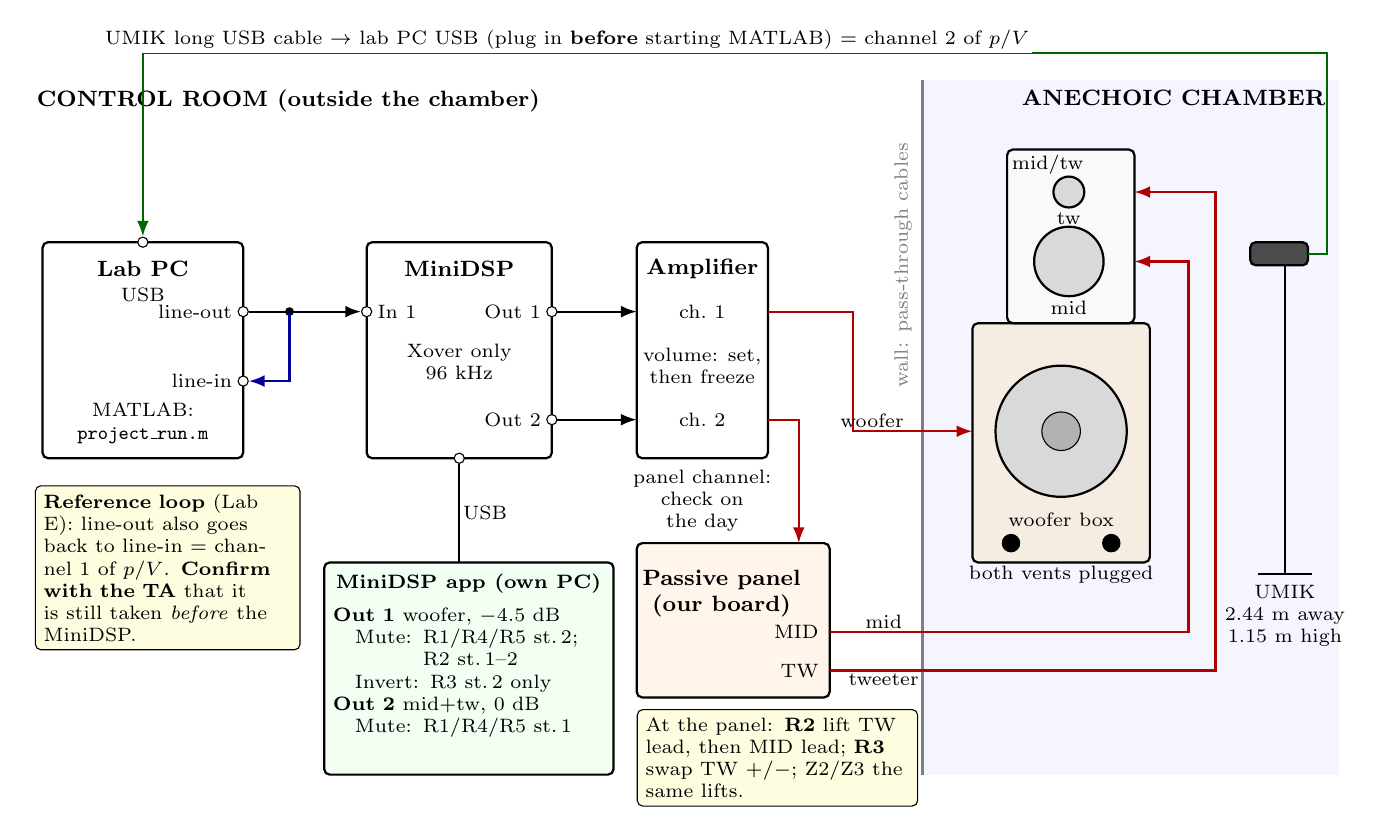
\begin{tikzpicture}[x=0.98cm,y=0.98cm,
  box/.style={draw, thick, rounded corners=2pt, fill=white},
  port/.style={circle, draw, fill=white, inner sep=1.3pt},
  lbl/.style={font=\scriptsize, inner sep=1pt},
  note/.style={draw, rounded corners=2pt, fill=yellow!12, font=\scriptsize, align=left, inner sep=3pt},
  sig/.style={thick, -{Latex[length=2mm]}},
  spk/.style={thick, -{Latex[length=2mm]}, red!70!black},
  every node/.style={font=\footnotesize}]
  % ---------------- regions
  \fill[blue!4] (11.6,0) rectangle (17.0,9.0);
  \draw[very thick, gray] (11.6,0) -- (11.6,9.0);
  \node[font=\footnotesize\bfseries, anchor=north west] at (0,9.0) {CONTROL ROOM (outside the chamber)};
  \node[font=\footnotesize\bfseries, anchor=north east] at (16.95,9.0) {ANECHOIC CHAMBER};
  \node[lbl, rotate=90, gray] at (11.35,6.6) {wall: pass-through cables};
  % ---------------- lab PC
  \draw[box] (0.2,4.1) rectangle (2.8,6.9);
  \node[font=\footnotesize\bfseries] at (1.5,6.55) {Lab PC};
  \node[lbl, align=center] at (1.5,4.55) {MATLAB:\\ \texttt{project\_run.m}};
  \node[port] (lo) at (2.8,6.0) {}; \node[lbl, anchor=east] at (2.7,6.0) {line-out};
  \node[port] (li) at (2.8,5.1) {}; \node[lbl, anchor=east] at (2.7,5.1) {line-in};
  \node[port] (usb) at (1.5,6.9) {}; \node[lbl, anchor=north] at (1.5,6.35) {USB};
  % reference loop
  \draw[thick] (lo) -- (3.4,6.0);
  \fill (3.4,6.0) circle (1.6pt);
  \draw[sig, blue!60!black] (3.4,6.0) -- (3.4,5.1) -- (li);
  \node[note, anchor=north west, text width=3.15cm] at (0.1,3.75)
    {\textbf{Reference loop} (Lab E): line-out also goes back to line-in = channel 1 of $p/V$.
     \textbf{Confirm with the TA} that it is still taken \emph{before} the MiniDSP.};
  % ---------------- MiniDSP
  \draw[box] (4.4,4.1) rectangle (6.8,6.9);
  \node[font=\footnotesize\bfseries] at (5.6,6.55) {MiniDSP};
  \node[lbl, align=center] at (5.6,5.35) {Xover only\\96 kHz};
  \node[port] (in1) at (4.4,6.0) {}; \node[lbl, anchor=west] at (4.5,6.0) {In 1};
  \node[port] (o1) at (6.8,6.0) {}; \node[lbl, anchor=east] at (6.7,6.0) {Out 1};
  \node[port] (o2) at (6.8,4.6) {}; \node[lbl, anchor=east] at (6.7,4.6) {Out 2};
  \node[port] (dusb) at (5.6,4.1) {};
  \draw[sig] (3.4,6.0) -- (in1);
  % ---------------- MiniDSP app PC
  \draw[box, fill=green!5] (3.85,0.0) rectangle (7.6,2.75);
  \node[font=\scriptsize\bfseries] at (5.72,2.47) {MiniDSP app (own PC)};
  \node[lbl, align=left, anchor=north west, text width=3.6cm] at (3.92,2.2)
    {\textbf{Out 1} woofer, $-4.5$ dB\\
     \quad Mute: R1/R4/R5 st.\,2;\\ \quad\phantom{Mute: }R2 st.\,1--2\\
     \quad Invert: R3 st.\,2 only\\
     \textbf{Out 2} mid+tw, 0 dB\\
     \quad Mute: R1/R4/R5 st.\,1};
  \draw[thick] (dusb) -- (5.6,2.75) node[lbl, pos=0.5, right] {USB};
  % ---------------- amplifier
  \draw[box] (7.9,4.1) rectangle (9.6,6.9);
  \node[font=\footnotesize\bfseries] at (8.75,6.55) {Amplifier};
  \node[lbl] at (8.75,6.0) {ch.~1};
  \node[lbl] at (8.75,4.6) {ch.~2};
  \node[lbl, align=center] at (8.75,5.3) {volume: set,\\then freeze};
  \draw[sig] (o1) -- (7.9,6.0);
  \draw[sig] (o2) -- (7.9,4.6);
  \node[lbl, align=center, text width=1.9cm, fill=white] at (8.75,3.55) {panel channel:\\check on the day};
  % ---------------- passive panel
  \draw[box, fill=orange!8] (7.9,1.0) rectangle (10.4,3.0);
  \node[font=\footnotesize\bfseries, align=center] at (9.0,2.35) {Passive panel\\(our board)};
  \node[lbl, anchor=east] at (10.3,1.85) {MID};
  \node[lbl, anchor=east] at (10.3,1.35) {TW};
  \draw[spk] (9.6,4.6) -- (10.0,4.6) -- (10.0,3.0);
  \node[note, anchor=north west, text width=3.35cm] at (7.9,0.85)
    {At the panel: \textbf{R2} lift TW lead, then MID lead; \textbf{R3} swap TW $+/-$; Z2/Z3 the same lifts.};
  % ---------------- amp ch1 -> woofer
  \draw[spk] (9.6,6.0) -- (10.7,6.0) -- (10.7,4.45) -- (12.25,4.45);
  \node[lbl, anchor=south] at (10.95,4.45) {woofer};
  % ---------------- panel -> mid, tweeter
  \draw[spk] (10.4,1.85) -- (15.05,1.85) -- (15.05,6.65) -- (14.35,6.65);
  \draw[spk] (10.4,1.35) -- (15.4,1.35) -- (15.4,7.55) -- (14.35,7.55);
  \node[lbl, anchor=south] at (11.1,1.85) {mid};
  \node[lbl, anchor=north] at (11.1,1.35) {tweeter};
  % ---------------- boxes in the chamber
  \draw[box, fill=brown!15] (12.25,2.75) rectangle (14.55,5.85);
  \draw[thick, fill=gray!30] (13.4,4.45) circle (0.85);
  \draw[fill=gray!60] (13.4,4.45) circle (0.25);
  \node[lbl] at (13.4,3.3) {woofer box};
  \fill[black] (12.75,3.0) circle (0.12); \fill[black] (14.05,3.0) circle (0.12);
  \node[lbl, anchor=north] at (13.4,2.75) {both vents plugged};
  \draw[box, fill=gray!5] (12.7,5.85) rectangle (14.35,8.1);
  \draw[thick, fill=gray!30] (13.5,6.65) circle (0.45);
  \draw[thick, fill=gray!30] (13.5,7.55) circle (0.2);
  \node[lbl, anchor=west] at (12.72,7.9) {mid/tw};
  \node[lbl] at (13.5,7.2) {tw};
  \node[lbl] at (13.5,6.05) {mid};
  % ---------------- UMIK
  \draw[thick] (16.3,2.6) -- (16.3,6.75);
  \draw[thick] (15.95,2.6) -- (16.65,2.6);
  \draw[box, fill=black!70] (15.85,6.6) rectangle (16.6,6.9);
  \node[lbl, align=center, anchor=north] at (16.3,2.5) {UMIK\\2.44 m away\\1.15 m high};
  % UMIK USB back to the PC
  \draw[sig, green!40!black] (16.6,6.75) -- (16.85,6.75) -- (16.85,9.35) -- (1.5,9.35) -- (usb);
  \node[lbl, fill=white, anchor=south] at (7.0,9.35) {UMIK long USB cable $\to$ lab PC USB (plug in \textbf{before} starting MATLAB) = channel 2 of $p/V$};
\end{tikzpicture}

\caption{Wiring in the chamber session. The script computes $H = p/V$ from the UMIK (channel 2) and the
line-in reference (channel 1), as in Lab E. Everything except the boxes and the microphone stays in the
control room, including the passive panel, so muting and lead lifting never need the chamber door. The
Project Guide says one amplifier channel feeds the panel and the other goes straight to the chamber:
check on the day which one, and make sure MiniDSP Output~2 drives the panel channel.}
\label{fig:chain}
\end{figure}

\begin{warnbox}[The one thing to confirm with Vicente before measuring]
Our scripts assume the line-in reference is still taken from the sound card line-out \emph{before} the
MiniDSP, as in Lab E. Then $H$ is the response of the whole system (MiniDSP + amplifier + board +
drivers), which is what the model curves show. If the reference is now tapped after the MiniDSP or after
the amplifier, the measured curves are not the system response: stop and adapt the plan with him.
\end{warnbox}

\subsection{The passive board (person A, 13:15--13:35)}\label{sec:board}

The board sits on amplifier channel~2. Both branches start at the amplifier $+$ terminal; every shunt
part goes to the common return ($-$). Wire both drivers red to $+$.

\begin{figure}[H]
\centering
% The passive board as physically wired (top view sketch). Terminal names are ours.
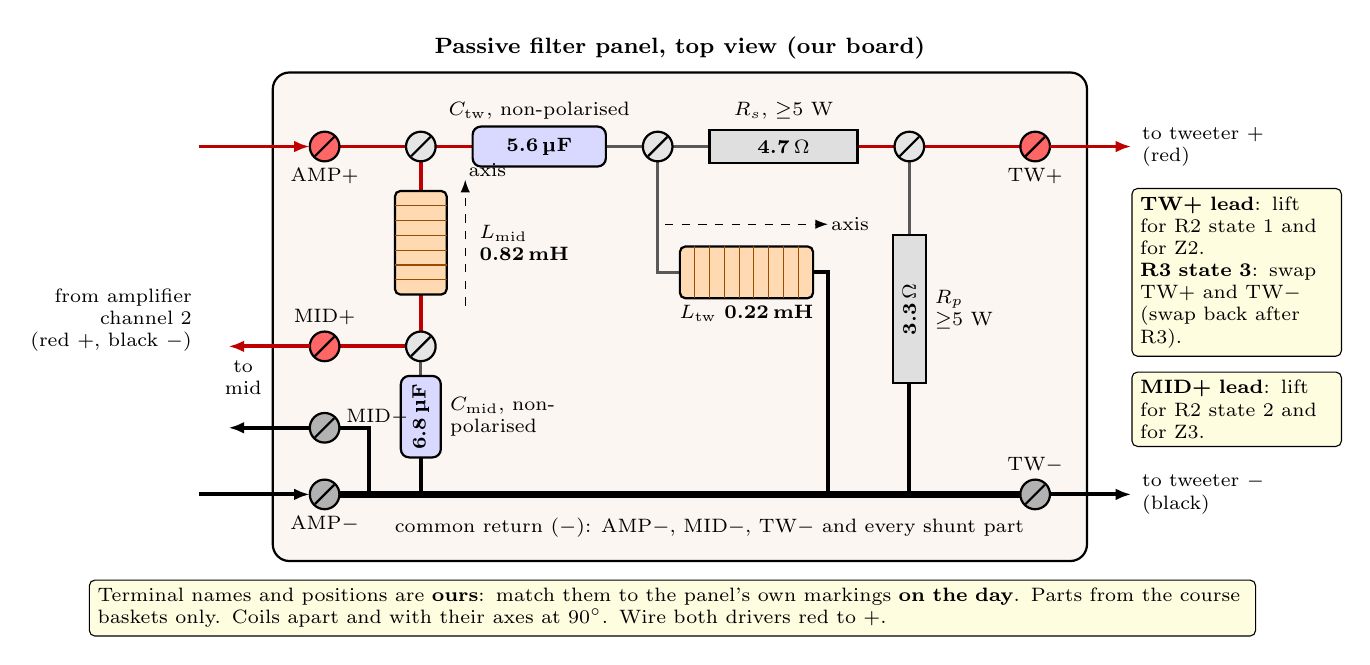
\begin{tikzpicture}[x=0.94cm,y=0.94cm,
  lbl/.style={font=\scriptsize, inner sep=1pt},
  val/.style={font=\scriptsize\bfseries, inner sep=1pt},
  note/.style={draw, rounded corners=2pt, fill=yellow!12, font=\scriptsize, align=left, inner sep=3pt},
  wp/.style={line width=1.4pt, red!75!black},
  wn/.style={line width=1.4pt, black},
  wi/.style={line width=1.2pt, black!65},
  every node/.style={font=\footnotesize}]
  \newcommand{\screw}[2]{\draw[fill=#2, thick] (#1) circle (0.2);
     \draw[thick] ($(#1)+(-0.13,-0.13)$) -- ($(#1)+(0.13,0.13)$);}
  % board
  \draw[rounded corners=6pt, thick, fill=brown!7] (0,0) rectangle (11,6.6);
  \node[font=\footnotesize\bfseries, anchor=south] at (5.5,6.65) {Passive filter panel, top view (our board)};
  % ground bus
  \draw[wn, line width=2.4pt] (0.7,0.9) -- (10.3,0.9);
  \node[lbl] at (5.9,0.45) {common return ($-$): AMP$-$, MID$-$, TW$-$ and every shunt part};
  % ---------- wires
  \draw[wp] (0.7,5.6) -- (2.0,5.6) -- (2.7,5.6);          % AMP+ -> A -> C_tw
  \draw[wi] (4.5,5.6) -- (5.2,5.6) -- (5.9,5.6);          % C_tw -> J -> Rs
  \draw[wp] (7.9,5.6) -- (8.6,5.6) -- (10.3,5.6);         % Rs -> T -> TW+
  \draw[wp] (2.0,5.6) -- (2.0,5.0);                       % A -> L_mid
  \draw[wp] (2.0,3.6) -- (2.0,2.9) -- (0.7,2.9);          % L_mid -> M -> MID+
  \draw[wi] (2.0,2.9) -- (2.0,2.5);                       % M -> C_mid
  \draw[wn] (2.0,1.4) -- (2.0,0.9);                       % C_mid -> bus
  \draw[wn] (0.7,1.8) -- (1.3,1.8) -- (1.3,0.9);          % MID- -> bus
  \draw[wi] (5.2,5.6) -- (5.2,3.9) -- (5.5,3.9);          % J -> L_tw
  \draw[wn] (7.3,3.9) -- (7.5,3.9) -- (7.5,0.9);          % L_tw -> bus
  \draw[wi] (8.6,5.6) -- (8.6,4.4);                       % T -> Rp
  \draw[wn] (8.6,2.4) -- (8.6,0.9);                       % Rp -> bus
  % ---------- parts
  % C_tw
  \draw[thick, fill=blue!15, rounded corners=3pt] (2.7,5.33) rectangle (4.5,5.87);
  \node[val] at (3.6,5.6) {5.6\,\textmu F};
  \node[lbl, anchor=south] at (3.6,5.92) {$C_\mathrm{tw}$, non-polarised};
  % Rs
  \draw[thick, fill=gray!25] (5.9,5.38) rectangle (7.9,5.82);
  \node[val] at (6.9,5.6) {4.7\,$\Omega$};
  \node[lbl, anchor=south] at (6.9,5.92) {$R_s$, $\geq$5 W};
  % L_tw: horizontal axis
  \draw[thick, fill=orange!30, rounded corners=2pt] (5.5,3.55) rectangle (7.3,4.25);
  \foreach \x in {5.7,5.9,...,7.15} \draw[orange!60!black] (\x,3.55) -- (\x,4.25);
  \draw[dashed, -{Latex[length=1.6mm]}] (5.3,4.55) -- (7.5,4.55) node[lbl, right] {axis};
  \node[lbl, anchor=north] at (6.4,3.5) {$L_\mathrm{tw}$ \textbf{0.22\,mH}};
  % Rp: vertical
  \draw[thick, fill=gray!25] (8.38,2.4) rectangle (8.82,4.4);
  \node[val, rotate=90] at (8.6,3.4) {3.3\,$\Omega$};
  \node[lbl, anchor=west, align=left] at (8.9,3.4) {$R_p$\\$\geq$5 W};
  % L_mid: vertical axis
  \draw[thick, fill=orange!30, rounded corners=2pt] (1.65,3.6) rectangle (2.35,5.0);
  \foreach \y in {3.8,4.0,...,4.85} \draw[orange!60!black] (1.65,\y) -- (2.35,\y);
  \draw[dashed, -{Latex[length=1.6mm]}] (2.6,3.45) -- (2.6,5.15) node[lbl, above right] {axis};
  \node[lbl, anchor=west, align=left] at (2.75,4.3) {$L_\mathrm{mid}$\\\textbf{0.82\,mH}};
  % C_mid: vertical
  \draw[thick, fill=blue!15, rounded corners=3pt] (1.73,1.4) rectangle (2.27,2.5);
  \node[val, rotate=90] at (2.0,1.95) {6.8\,\textmu F};
  \node[lbl, anchor=west, align=left] at (2.35,1.95) {$C_\mathrm{mid}$, non-\\polarised};
  % ---------- screws (internal junctions) and terminals
  \screw{2.0,5.6}{gray!20} \screw{5.2,5.6}{gray!20} \screw{8.6,5.6}{gray!20} \screw{2.0,2.9}{gray!20}
  \screw{0.7,5.6}{red!60} \screw{0.7,2.9}{red!60} \screw{0.7,1.8}{gray!60} \screw{0.7,0.9}{gray!60}
  \screw{10.3,5.6}{red!60} \screw{10.3,0.9}{gray!60}
  \node[lbl, anchor=north] at (0.7,5.35) {AMP+};
  \node[lbl, anchor=south] at (0.7,3.15) {MID+};
  \node[lbl, anchor=west] at (0.95,1.95) {MID$-$};
  \node[lbl, anchor=north] at (0.7,0.65) {AMP$-$};
  \node[lbl, anchor=north] at (10.3,5.35) {TW+};
  \node[lbl, anchor=south] at (10.3,1.15) {TW$-$};
  % ---------- leads leaving the board
  \draw[wp, {Latex[length=2mm]}-] (0.5,5.6) -- (-1.0,5.6);
  \draw[wn, {Latex[length=2mm]}-] (0.5,0.9) -- (-1.0,0.9);
  \node[lbl, align=right, anchor=east] at (-1.05,3.25) {from amplifier\\channel 2\\(red +, black $-$)};
  \draw[wp, -{Latex[length=2mm]}] (0.5,2.9) -- (-0.6,2.9);
  \draw[wn, -{Latex[length=2mm]}] (0.5,1.8) -- (-0.6,1.8);
  \node[lbl, align=center, fill=white, anchor=north] at (-0.4,2.75) {to\\mid};
  \draw[wp, -{Latex[length=2mm]}] (10.5,5.6) -- (11.6,5.6);
  \draw[wn, -{Latex[length=2mm]}] (10.5,0.9) -- (11.6,0.9);
  \node[lbl, align=left, anchor=west] at (11.7,5.6) {to tweeter +\\(red)};
  \node[lbl, align=left, anchor=west] at (11.7,0.9) {to tweeter $-$\\(black)};
  % ---------- what to lift / swap
  \node[note, anchor=west, text width=2.45cm] at (11.6,3.9)
    {\textbf{TW+ lead}: lift for R2 state 1 and for Z2.\\
     \textbf{R3 state 3}: swap TW+ and TW$-$ (swap back after R3).};
  \node[note, anchor=west, text width=2.45cm] at (11.6,2.05)
    {\textbf{MID+ lead}: lift for R2 state 2 and for Z3.};
  \node[note, anchor=north, text width=14.6cm] at (5.4,-0.25)
    {Terminal names and positions are \textbf{ours}: match them to the panel's own markings \textbf{on the day}.
     Parts from the course baskets only. Coils apart and with their axes at \ang{90}. Wire both drivers red to +.};
\end{tikzpicture}


\vspace{5mm}
\begin{circuitikz}[european resistors, american inductors, scale=0.9, transform shape]
  \draw (0,-2) node[ground]{} to[sV, l=amp ch.~2] (0,0) -- (1.2,0) node[circ]{};
  % midrange: LP2
  \draw (1.2,0) -- (1.2,1.6) to[L, l=$L_\mathrm{mid}$, a=\SI{0.82}{mH}] (4.4,1.6) node[circ]{}
        to[C, l_=$C_\mathrm{mid}$, a^=\SI{6.8}{\micro F}] (4.4,-0.4) node[ground]{};
  \draw (4.4,1.6) -- (10.5,1.6) to[R, l=midrange, *-] (10.5,-0.4) node[ground]{};
  \node[font=\small, anchor=east] at (10.35,1.25) {red $+$};
  % tweeter: HP2 + L-pad
  \draw (1.2,0) -- (1.2,-2.4) to[C, l=$C_\mathrm{tw}$, a=\SI{5.6}{\micro F}] (4.4,-2.4) node[circ]{}
        to[L, l_=$L_\mathrm{tw}$, a^=\SI{0.22}{mH}] (4.4,-4.4) node[ground]{};
  \draw (4.4,-2.4) to[R, l=$R_s$, a=\SI{4.7}{\ohm}] (7.4,-2.4) node[circ]{}
        to[R, l_=$R_p$, a^=\SI{3.3}{\ohm}] (7.4,-4.4) node[ground]{};
  \draw (7.4,-2.4) -- (10.5,-2.4) to[R, l=tweeter, *-] (10.5,-4.4) node[ground]{};
  \node[font=\small, anchor=east] at (10.35,-2.75) {red $+$};
  \node[font=\small\itshape, anchor=west] at (0.95,2.5) {midrange low-pass, 2nd order (LC corner 2131 Hz)};
  \node[font=\small\itshape, anchor=west] at (1.4,-1.25) {tweeter high-pass, 2nd order (LC corner 4534 Hz) + L-pad};
  \draw[dashed, rounded corners] (0.8,2.9) rectangle (8.4,-4.95);
  \node[font=\small, anchor=north east] at (8.4,-5.0) {passive board};
\end{circuitikz}
\caption{The passive board. Top: how to wire it (a top-view sketch; the terminal names are ours, match
them to the panel on the day). Bottom: the same circuit as a schematic. All values are single parts from
Appendix~1, Table~1 of the Project Guide. Acoustic crossovers in the model: woofer/midrange \SI{324}{Hz}
(MiniDSP), midrange/tweeter \SI{3.76}{kHz} (this board). The L-pad lowers the tweeter by about
\SI{11}{dB}.}
\label{fig:board}
\end{figure}

\begin{table}[H]
\centering\small
\begin{tabularx}{\textwidth}{@{}l l l L@{}}
\toprule
Part & Value & Where it goes & Check the basket part \\
\midrule
$L_\mathrm{mid}$ & \SI{0.82}{mH} & series, amp $+$ $\to$ midrange $+$ & carries up to $\sim$\SI{1.9}{A} rms at \SI{10}{W} \\
$C_\mathrm{mid}$ & \SI{6.8}{\micro F} & across the midrange ($+$ to $-$) & \textbf{non-polarised} (film or bipolar), $\geq$\SI{25}{V} \\
$C_\mathrm{tw}$ & \SI{5.6}{\micro F} & series, amp $+$ $\to$ tweeter node & \textbf{non-polarised}, $\geq$\SI{25}{V} \\
$L_\mathrm{tw}$ & \SI{0.22}{mH} & tweeter node $\to$ return & -- \\
$R_s$ & \SI{4.7}{\ohm} & series, node $\to$ tweeter $+$ & \textbf{power resistor, $\geq$\SI{5}{W}} \\
$R_p$ & \SI{3.3}{\ohm} & across the tweeter & power resistor, $\geq$\SI{5}{W} \\
\bottomrule
\end{tabularx}
\end{table}

\begin{itemize}[leftmargin=14pt]
\item[\tick] \textbf{Where the parts come from:} only the course baskets (Project Guide 3.2), values from
  Appendix~1, Table~1. There are at least two parts of each value. Do not combine parts to make an
  in-between value; all six of our values are in the table. Return unused parts and every banana cable
  to their basket afterwards, and report parts that are running low, missing or faulty.
\item[\tick] Measure each part with the LCR meter if the lab has one, and each coil's DC resistance with
  the multimeter. Write the numbers into \file{project_dims.m} (\cmd{d.board}, \cmd{d.coil_dcr}). For
  reference: coil resistance of 0.3/0.6/1.0\,$\Omega$ per mH lowers the summed response by at most
  0.23/0.45/0.74\,dB, and 400 random boards within the part tolerances stayed inside a \SI{1.7}{dB} band.
\item[\tick] Keep the two coils apart and at right angles to each other (so one does not pick up the
  other's field).
\item[\tick] Note which panel (1--10) we use: \cmd{d.panel_no}. The load the board puts on amplifier
  channel 2 never drops below \SI{4.4}{\ohm} (model).
\end{itemize}

\subsection{The MiniDSP (person B, 13:15--13:35)}\label{sec:dsp}

Steps from the Project Guide, section 3.1, with our values:
\begin{enumerate}[leftmargin=16pt]
\item Open the MiniDSP software on its PC and click \emph{Connect}.
\item \textbf{Routing matrix:} only \emph{Input 1 $\to$ Output 1} and \emph{Input 1 $\to$ Output 2} active.
\item \textbf{Outputs:} only outputs 1 and 2 are used. On both, only \emph{Xover} is active: PEQ, Comp and
  FIR must show as bypassed (we cannot reproduce them in LTspice).
\item \textbf{Output 1 (woofer):} Xover $\to$ \emph{Advanced}, delete the contents of the text window,
  paste the whole of \file{Project/Final design/data/dsp/MiniDSP_woofer_out1.txt} (open it in Notepad on
  the stick and copy from there, never from this PDF: hidden characters), click \emph{Process}. It is two
  identical Butterworth low-pass biquads at \SI{325}{Hz} = one LR4 low-pass.
\item \textbf{Output 2 (mid + tweeter):} same with \file{MiniDSP_midtw_out2.txt} (the LR4 high-pass).
  Synchronise the configuration with the DSP card if the app asks.
\item \textbf{Gains:} Output 1 \SI{-4.5}{dB}, Output 2 \SI{0}{dB}. Invert off on both. Delay 0 on both
  (the ``$d = \SI{-1.15}{m}$'' in our report is only the distance correction for drawing phase plots,
  not a delay to type in).
\item \textbf{Sample rate:} the coefficients only give \SI{325}{Hz} at \SI{96}{kHz}. Check the plugin
  says 96~kHz (\cmd{d.minidsp_fs}).
\item Save the configuration (slot and file); write the names in \cmd{d.minidsp_cfg}.
\end{enumerate}

\begin{table}[H]
\centering\small
\begin{tabular}{@{}ll@{}}
\toprule
Setting & Value \\
\midrule
Routing & Input 1 $\to$ Output 1, Input 1 $\to$ Output 2, nothing else \\
PEQ, Comp, FIR & bypassed on both outputs \\
Output 1 Xover, Advanced & \file{MiniDSP_woofer_out1.txt} (LR4 low-pass \SI{325}{Hz}), Process \\
Output 2 Xover, Advanced & \file{MiniDSP_midtw_out2.txt} (LR4 high-pass \SI{325}{Hz}), Process \\
Gain & Output 1 \SI{-4.5}{dB}, Output 2 \SI{0}{dB} \\
Invert / polarity & off on both (R3 ticks Out 1 for one state, then untick) \\
Delay & 0 on both \\
Sample rate & \SI{96}{kHz} \\
\bottomrule
\end{tabular}
\caption{MiniDSP settings. The coefficient texts are in Appendix~\ref{app:dsp}.}
\end{table}

\subsection{Placing the system and the microphone (person C, 13:15--13:35)}\label{sec:place}
\begin{figure}[H]
\centering
% Placement in the anechoic chamber, as in Lab E (side view roughly to scale, 1 m = 3.2 cm)
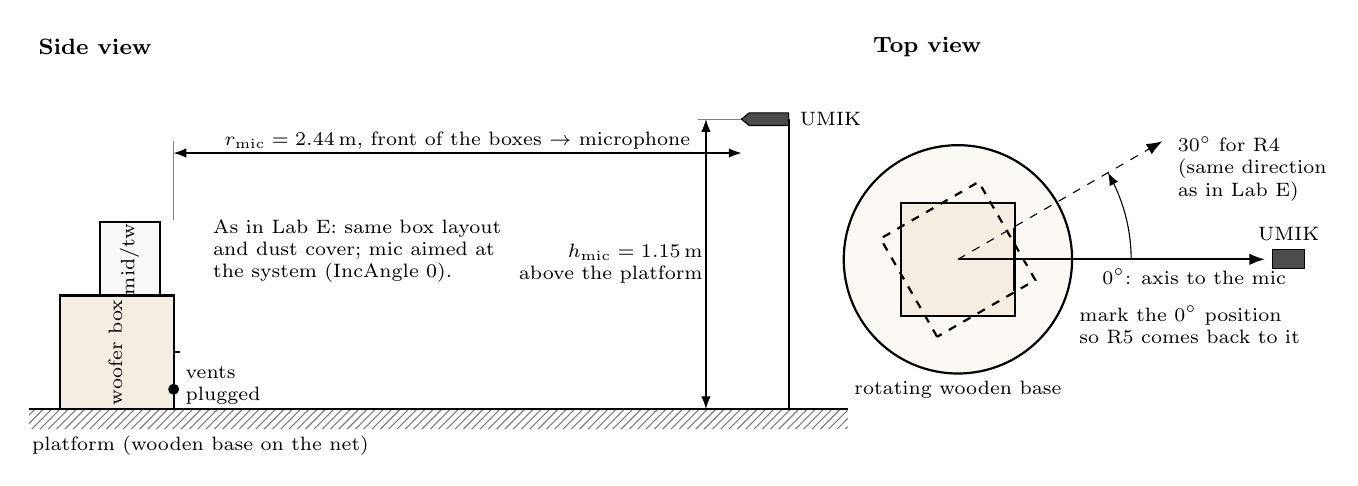
\begin{tikzpicture}[x=1cm,y=1cm,
  lbl/.style={font=\scriptsize, inner sep=1pt},
  dim/.style={{Latex[length=1.6mm]}-{Latex[length=1.6mm]}, thin},
  every node/.style={font=\footnotesize}]
  % ---------- side view
  \node[font=\footnotesize\bfseries, anchor=west] at (0,4.6) {Side view};
  \fill[pattern=north east lines, pattern color=gray] (0,-0.25) rectangle (10.4,0);
  \draw[thick] (0,0) -- (10.4,0);
  \node[lbl, anchor=north west] at (0,-0.3) {platform (wooden base on the net)};
  \draw[thick, fill=brown!15] (0.4,0) rectangle (1.84,1.44);
  \node[lbl, rotate=90] at (1.1,0.72) {woofer box};
  \fill (1.84,0.25) circle (0.07);
  \node[lbl, anchor=west, align=left] at (1.95,0.3) {vents\\plugged};
  \draw[thick, fill=gray!5] (0.9,1.44) rectangle (1.67,2.37);
  \node[lbl, rotate=90] at (1.28,1.9) {mid/tw};
  \draw[thick] (1.84,0.72) -- (1.92,0.72);
  % microphone on a stand
  \draw[thick] (9.65,0) -- (9.65,3.68);
  \draw[thick] (9.3,0) -- (10.0,0);
  \draw[fill=black!70] (9.65,3.6) -- (9.15,3.6) -- (9.05,3.68) -- (9.15,3.76) -- (9.65,3.76) -- cycle;
  \node[lbl, anchor=west] at (9.75,3.68) {UMIK};
  % dimensions
  \draw[dim] (1.84,3.25) -- (9.05,3.25) node[lbl, midway, above, fill=white] {$r_\mathrm{mic} = \SI{2.44}{m}$, front of the boxes $\to$ microphone};
  \draw[thin, gray] (1.84,2.4) -- (1.84,3.4);
  \draw[dim] (8.6,0) -- (8.6,3.68) node[lbl, midway, left, fill=white, align=right] {$h_\mathrm{mic} = \SI{1.15}{m}$\\above the platform};
  \draw[thin, gray] (8.5,3.68) -- (9.05,3.68);
  \node[lbl, align=left, anchor=west, text width=4.0cm] at (2.3,2.0) {As in Lab E: same box layout and dust cover; mic aimed at the system (IncAngle 0).};
  % ---------- top view
  \begin{scope}[xshift=11.8cm, yshift=1.9cm]
  \node[font=\footnotesize\bfseries, anchor=west] at (-1.2,2.7) {Top view};
  \draw[thick, fill=brown!5] (0,0) circle (1.45);
  \node[lbl, anchor=north] at (0,-1.5) {rotating wooden base};
  % 0 deg
  \draw[thick, fill=brown!15] (-0.72,-0.72) rectangle (0.72,0.72);
  \draw[very thick] (0.72,-0.4) -- (0.72,0.4);
  \draw[-{Latex[length=2mm]}, thick] (0,0) -- (3.9,0);
  \node[lbl, anchor=north] at (3.0,-0.08) {\ang{0}: axis to the mic};
  % 30 deg (dashed)
  \begin{scope}[rotate=30]
    \draw[dashed, thick] (-0.72,-0.72) rectangle (0.72,0.72);
    \draw[dashed, -{Latex[length=2mm]}] (0,0) -- (3.0,0);
  \end{scope}
  \draw[-{Latex[length=1.6mm]}] (2.2,0) arc (0:30:2.2);
  \node[lbl, anchor=west, align=left] at (2.75,1.15) {\ang{30} for R4\\(same direction\\as in Lab E)};
  \draw[fill=black!70] (4.0,-0.12) rectangle (4.4,0.12);
  \node[lbl, anchor=south] at (4.2,0.2) {UMIK};
  \node[lbl, align=left, anchor=north west] at (1.5,-0.55) {mark the \ang{0} position\\so R5 comes back to it};
  \end{scope}
\end{tikzpicture}

\caption{Placement in the chamber, as in Lab E (side view roughly to scale). The microphone stays put all
session; only the wooden base turns for R4 and back for R5.}\label{fig:place}
\end{figure}
\begin{itemize}[leftmargin=14pt]
\item[\tick] Same placement as in Lab E, because the model curves are built from the Lab E data: mid/tweeter
  box on the woofer box in the Lab E position, microphone \SI{2.44}{m} from the front of the boxes and
  \SI{1.15}{m} above the platform, pointing at the system (IncAngle 0). Write the real numbers into
  \cmd{d.r_mic}, \cmd{d.h_mic}, \cmd{d.layout}.
\item[\tick] Both woofer vents plugged (``you may just cover the vents'', Task 3): the chamber is not valid
  below \SI{125}{Hz}, so the vent tuning is measured at the Lab D station instead. Filling stays in.
\item[\tick] Dust cover as in Lab E (\cmd{d.dust_cover}). Read the UMIK serial on its label
  (0329, 0332 or 0335; Lab E was 708-0332) and put it in \cmd{d.UmikSN}. Note the chamber temperature.
\item[\tick] Connect the woofer to amplifier channel 1 and the two board outputs to the midrange and the
  tweeter, red to $+$. Mark the \ang{0} position of the wooden base so R5 comes back to it.
\item[\tick] Plug the UMIK USB cable into the PC \textbf{before} MATLAB is started, or the routine does not
  find it.
\end{itemize}

\subsection{Files on the lab PC (13:35)}\label{sec:files}
\begin{enumerate}[leftmargin=16pt]
\item Copy the folder \file{Labs/} from the stick to the lab PC (for example \file{Desktop\Group10\Labs}).
  Copy the whole folder: the scripts find the course routines and the Lab D reference data by relative
  paths (\file{Labs/Lab E/matlab/course}, \file{Labs/Lab D/matlab}, \file{Labs/Lab D/data}).
\item Start MATLAB (UMIK already plugged in), \cmd{cd} to
  \file{Labs/Project/Final design/lab-day/matlab} and open \file{project_run.m}.
\item Click in section \textbf{0} and press \emph{Run Section} (Ctrl+Enter). It opens
  \file{project_dims.m}: fill in everything you have (Appendix~\ref{app:dims}) and save. Then it runs
  \cmd{test_project}, which simulates a whole run without hardware.
\end{enumerate}
\begin{checkbox}
\cmd{test_project} ends with \cmd{PASS}. If it prints \cmd{FAIL} or an error, the copy is incomplete:
copy \file{Labs/} again. New data will be saved in \file{lab-day/data/} as
\file{project_<tag>.mat} (a repeated tag gets \file{_2}, \file{_3}; nothing is ever overwritten).
\end{checkbox}

\subsection{Electrical check and level setting (13:40)}\label{sec:levels}
\textbf{Scope check of the MiniDSP.} Play a \SI{325}{Hz} sine from the lab PC, e.g. in MATLAB:
\begin{Verbatim}[fontsize=\small,frame=single,framesep=2mm]
fs = 48000; t = (0:10*fs-1)/fs; sound(0.1*sin(2*pi*325*t), fs)   % 10 s at 325 Hz
\end{Verbatim}
and look at the MiniDSP input and its two outputs on the scope (amplifier volume low).
\begin{checkbox}[What the scope should show]
Output 1 = input \SI{-10.5}{dB} (factor 0.30: \SI{-6}{dB} from the filter at its corner, \SI{-4.5}{dB}
gain). Output 2 = input \SI{-6.0}{dB} (factor 0.50). Output 1 and Output 2 \textbf{in phase} (an LR4 pair is
\ang{360} apart at the crossover). The ratio Out\,1/Out\,2 = \SI{-4.5}{dB} is the robust number, even if
the input gain is not 0~dB.
\end{checkbox}

\textbf{Trial run for the amplifier volume.} Start with the volume low and run once, outside
\file{project_run.m}, with one state (about a minute):
\begin{Verbatim}[fontsize=\small,frame=single,framesep=2mm]
m = measure_project('trial_0', 0, {'all'}, 'note', 'level trial');
\end{Verbatim}
Raise the volume until the UMIK peak printed after the run is well above 0.01 and below 0.95 (no
warnings), and the measured curve is smooth up to \SI{20}{kHz}. Then write the knob position in
\cmd{d.amp_volume} and \textbf{do not touch the volume or the microphone again} until R5 is done.

\subsection{Procedure: the five runs (13:50--14:40)}

One run measures one to three states in one go. Between two states the routine plays about
\SI{30}{s} of beeps: that is when you switch. States inside one run share a phase reference; separate
runs do not (the UMIK has its own USB clock), so phases are only compared within a run. Muting happens in
the MiniDSP app; lead swapping at the board, outside the chamber. After every run the script saves the
file, prints the peaks, plots the measured curves on top of the model (dashed, shifted by a fitted level)
and prints the checks below.

\begin{table}[H]
\centering\small
\begin{tabularx}{\textwidth}{@{}l c l L@{}}
\toprule
Run & Angle & States (switch during the beeps) & What it proves \\
\midrule
R1 & \ang{0} & woofer $\to$ mid+tw $\to$ all & each channel against the model; channel balance; woofer + mid/tw = all \\
R2 & \ang{0} & mid $\to$ tw $\to$ all & the passive board, driver by driver \\
R3 & \ang{0} & all $\to$ woofer inverted $\to$ tweeter swapped & phase alignment: notches at \SI{329}{Hz} and \SI{3.9}{kHz} \\
R4 & \ang{30} & woofer $\to$ mid+tw $\to$ all & off-axis, against the Lab E \ang{30} model \\
R5 & \ang{0} & woofer $\to$ mid+tw $\to$ all & repeat of R1: drift and placement \\
\bottomrule
\end{tabularx}
\end{table}

\begin{runbox}{R1 -- on axis, woofer / mid+tweeter / all \hfill \normalfont\file{project_run.m}, section R1}
\textbf{Before:} Output 2 \textbf{muted} in the app. \quad
\textbf{Beeps 1:} unmute Output 2, mute Output 1. \quad
\textbf{Beeps 2:} unmute Output 1.\\
Runs \cmd{measure_project('R1_split_0', 0, {'woofer','midtw','all'}, 'note','reference run')}.
\begin{checkbox}
\begin{Verbatim}[fontsize=\footnotesize]
R1_split_0  (0 deg)
  woofer  level offset vs model   +x.x dB, shape error (rms, 1/6 oct) 1.x dB
  midtw   level offset vs model   +x.x dB, shape error (rms, 1/6 oct) 1.x dB
  all     level offset vs model   +x.x dB, shape error (rms, 1/6 oct) 1.x dB
  woofer - midtw offset: +0.x dB (want within +-1 dB; else adjust the Out 1 gain by ...)
  sum check |woofer+midtw| vs |all|: worst 0.xx dB (1/6 oct, 150 Hz-15 kHz)
\end{Verbatim}
\begin{itemize}[leftmargin=12pt]
\item The \textbf{level offsets} themselves can be anything (amplifier volume, MiniDSP input gain). What
  matters is that \textbf{woofer and midtw agree within about \SI{1}{dB}}. If not, the two amplifier
  channels differ: change the Output 1 gain by the printed amount, note the new value in
  \cmd{d.minidsp_out1_gain}, and repeat R1 (the tag gets \file{_2}).
\item \textbf{Shape error} about 1--2~dB or less. \textbf{Sum check} under about \SI{0.5}{dB}; more means
  something moved or changed between the states: repeat the run.
\item The plot should look like the top panel of Figure~\ref{fig:on}: woofer and mid+tweeter cross near
  \SI{325}{Hz}, the sum is within $\pm 2$~dB from \SI{150}{Hz} to \SI{15}{kHz} (\SI{4.0}{dB} spread,
  1/6~octave).
\end{itemize}
\end{checkbox}
\end{runbox}

\begin{runbox}{R2 -- on axis, midrange / tweeter / all \hfill \normalfont section R2}
\textbf{Before:} Output 1 \textbf{muted}, \textbf{tweeter} lead off at the board. \quad
\textbf{Beeps 1:} tweeter lead on, midrange lead off. \quad
\textbf{Beeps 2:} midrange lead back on, unmute Output 1.\\
Runs \cmd{measure_project('R2_units_0', 0, {'mid','tw','all'})}.
\begin{checkbox}
Each driver's shape error is small (it is judged only where that driver is loud: midrange
600~Hz--2.5~kHz, tweeter 5--15~kHz). The midrange falls off above about \SI{4}{kHz} and the tweeter takes
over around \SI{3.8}{kHz} (Figure~\ref{fig:on}, top). If one driver is far off while the other is fine,
the fault is in that branch of the board (a part in the wrong place, a polarised capacitor, a loose
screw).
\end{checkbox}
\end{runbox}

\begin{runbox}{R3 -- polarity checks: all / woofer inverted / tweeter swapped \hfill \normalfont section R3}
\textbf{Before:} everything normal. \quad
\textbf{Beeps 1:} tick \textbf{Invert} on Output 1. \quad
\textbf{Beeps 2:} untick it, and swap the tweeter's $+$ and $-$ at the board.\\
Runs \cmd{measure_project('R3_flip_0', 0, {'all','flipW','flipT'})}.
\begin{checkbox}
\begin{Verbatim}[fontsize=\footnotesize]
  flipW: notch 3xx Hz, -2x.x dB below the normal sum      (model: 329 Hz, -20.9 dB)
  flipT: notch 3xxx Hz, -1x.x dB below the normal sum     (model: 3928 Hz, -14.2 dB)
\end{Verbatim}
A deep notch proves the two drivers are in phase at the crossover with normal wiring. A shallow notch or
one in the wrong place means a polarity or phase error: check red to $+$ on both drivers, and that the
Invert box really was ticked. Compare with Figure~\ref{fig:on}, bottom panel.
\end{checkbox}
\textbf{Afterwards: untick Invert (if still ticked) and swap the tweeter back.} Check both before R4.
\end{runbox}

\begin{runbox}{R4 -- \ang{30}, woofer / mid+tweeter / all \hfill \normalfont section R4}
Turn the wooden base \ang{30}, in the same direction as in Lab E. Same switching as R1.\\
Runs \cmd{measure_project('R4_split_30', 30, {'woofer','midtw','all'})} and compares with the \ang{30}
model (Figure~\ref{fig:off}).
\begin{checkbox}
Same checks as R1. Woofer -- midtw offset close to R1's value. Expected spread of the sum: about
\SI{6.3}{dB} (150~Hz--15~kHz, 1/6~octave); the top end rolls off above \SI{10}{kHz} (tweeter directivity).
\end{checkbox}
\end{runbox}

\begin{runbox}{R5 -- back to \ang{0}: repeat of R1 \hfill \normalfont section R5}
Turn back to the \ang{0} mark. Tweeter polarity normal, no invert. Same switching as R1.\\
Runs \cmd{measure_project('R5_repeat_0', 0, {'woofer','midtw','all'}, 'note','repeat of R1')} and
compares the ``all'' curve with R1.
\begin{checkbox}
\begin{Verbatim}[fontsize=\footnotesize]
R5 vs R1, all three: median +0.0x dB, worst 0.x dB
\end{Verbatim}
Median within a few tenths of a dB. A bigger shift means the system, the microphone or the volume moved
during the session; write it down (it is the uncertainty of the whole series).
\end{checkbox}
\end{runbox}

\textbf{Section 6 (optional, 14:40).} If R1 asked for a different Output 1 gain, or another change is tried,
run it with a new tag and a note saying exactly what changed, e.g.
\begin{Verbatim}[fontsize=\small,frame=single,framesep=2mm]
m = measure_project('R6_gain_0', 0, {'woofer','midtw','all'}, 'note', 'Out 1 gain -3.5 dB');
\end{Verbatim}

\subsection{Before leaving the chamber (14:50)}
\begin{itemize}[leftmargin=14pt]
\item[\tick] Save the MiniDSP configuration (slot and file); copy the file to the stick. The listening test
  and the demo start from it.
\item[\tick] Photograph the board from above, with the part values readable (report).
\item[\tick] Copy \file{Labs/Project/Final design/lab-day/data/} to the stick, into the same path.
  Check that the files open on the stick.
\item[\tick] Untick Invert, tweeter wired normally, vent plugs still in.
\item[\tick] Return unused parts and banana cables to their baskets. Take the board and the system to
  the Lab D station (careful with the wedges and the drivers).
\end{itemize}

% ======================================================================
\section{Part 2 -- Zi/Nfield station (Lab D setup), 15:00--17:00}

This is the Lab D setup, not the MiniDSP chain: the NI card's AO0 drives the amplifier, the amplifier
drives the load through the series resistor on the circuit connection board, AI0 reads the amplifier
voltage and AI1 the load voltage (for impedance) or the Nexus output (for near field). The impedance
is
\[
Z_L = R\,\frac{V_\mathrm{load}/V_\mathrm{amp}}{1 - V_\mathrm{load}/V_\mathrm{amp}} ,
\]
computed by \file{zinf_calc.m}. Two Lab D lessons are built into the scripts: $R$ must be the
\textbf{multimeter value of the series resistor} (about \SI{32.9}{\ohm}, never $R_E$), and when AI0 sits
on a DC offset of several volts (the amplifier's output stage; in Lab D it read half the amplifier
voltage), the script uses $V_\mathrm{amp} = 2\cdot\mathrm{AI0}$ and says so.

\begin{figure}[H]
\centering
% Zi/Nfield station wiring (Lab D setup). Channels from the Lab D description and meas_mag_spec2_LabD.m:
% AO0 -> amplifier; AI0 = amplifier output (V_amp); AI1 = load voltage (impedance) or Nexus output (near field).
\begin{circuitikz}[x=1cm,y=1cm, european resistors,
  box/.style={draw, thick, rounded corners=2pt, fill=white},
  port/.style={circle, draw, fill=white, inner sep=1.3pt},
  lbl/.style={font=\scriptsize, inner sep=1pt},
  note/.style={draw, rounded corners=2pt, fill=yellow!12, font=\scriptsize, align=left, inner sep=3pt},
  every node/.style={font=\footnotesize}]
  \newcommand{\cut}[1]{\node[red!70!black, font=\large\bfseries] at (#1) {$\times$};}
  % ======================= (a) impedance
  \node[font=\footnotesize\bfseries, anchor=west] at (0,4.25) {(a) Impedance, Z1--Z4: series resistor in};
  \draw[box] (0,0.4) rectangle (2.4,3.7);
  \node[font=\footnotesize\bfseries, align=center] at (1.1,3.2) {NI-4431\\[-1pt]\scriptsize(lab PC)};
  \node[port] (ao) at (2.4,2.9) {}; \node[lbl, anchor=east] at (2.3,2.9) {AO0};
  \node[port] (a0) at (2.4,1.8) {}; \node[lbl, anchor=east] at (2.3,1.8) {AI0};
  \node[port] (a1) at (2.4,0.9) {}; \node[lbl, anchor=east] at (2.3,0.9) {AI1};
  \draw[box] (3.3,2.5) rectangle (5.0,3.7);
  \node[font=\footnotesize\bfseries] at (4.15,3.35) {Amplifier};
  \draw[thick, -{Latex[length=2mm]}] (ao) -- (3.3,2.9);
  \draw (5.0,2.9) to[short, -*] (5.9,2.9) to[R, l=$R \approx \SI{33}{\ohm}$, a={multimeter value, e.g. 32.9}] (8.6,2.9)
        to[short, -*] (9.3,2.9) -- (10.3,2.9);
  \draw (4.75,2.5) node[ground]{};
  \node[lbl, anchor=south] at (5.45,2.95) {$V_\mathrm{amp}$};
  \node[lbl, anchor=south] at (9.75,2.95) {$V_\mathrm{load}$};
  \draw[thick, blue!60!black, -{Latex[length=2mm]}] (5.9,2.9) -- (5.9,1.8) -- (a0);
  \draw[thick, blue!60!black, -{Latex[length=2mm]}] (9.3,2.9) -- (9.3,0.9) -- (a1);
  \node[lbl, fill=white] at (4.2,1.8) {AI0 = $V_\mathrm{amp}$ (before R)};
  \node[lbl, fill=white] at (6.6,0.9) {AI1 = $V_\mathrm{load}$ (after R)};
  % load: our board with the two drivers
  \draw[box, fill=orange!8] (10.3,1.4) rectangle (12.3,3.7);
  \node[font=\footnotesize\bfseries, align=center] at (11.35,3.25) {our board};
  \node[lbl, anchor=west] at (10.35,2.9) {AMP+};
  \node[lbl, anchor=west] at (10.35,1.8) {AMP$-$};
  \draw (10.3,1.8) -- (10.0,1.8) node[ground]{};
  \node[lbl, anchor=east] at (12.25,2.9) {TW};
  \node[lbl, anchor=east] at (12.25,1.8) {MID};
  \draw[thick, red!70!black] (12.3,2.9) -- (13.05,2.9); \draw[thick, red!70!black] (13.45,2.9) -- (14.2,2.9);
  \draw[thick, red!70!black] (12.3,1.8) -- (13.05,1.8); \draw[thick, red!70!black] (13.45,1.8) -- (14.2,1.8);
  \cut{13.25,2.9} \cut{13.25,1.8}
  \node[lbl, anchor=south, red!70!black] at (13.25,3.05) {lift for Z2};
  \node[lbl, anchor=north, red!70!black] at (13.25,1.6) {lift for Z3};
  \draw[box] (14.2,2.6) rectangle (15.4,3.2); \node[lbl] at (14.8,2.9) {tweeter};
  \draw[box] (14.2,1.5) rectangle (15.4,2.1); \node[lbl] at (14.8,1.8) {midrange};
  \node[note, anchor=north west, text width=5.3cm] at (10.0,1.15)
    {Z1: as drawn. Z2: TW lead lifted. Z3: MID lead lifted.\\
     \textbf{Z4}: the \textbf{woofer} straight on R instead of the board (one vent open at 160 mm, the other plugged, filling in).};
  % ======================= (b) near field
  \begin{scope}[yshift=-5.6cm]
  \node[font=\footnotesize\bfseries, anchor=west] at (0,4.25) {(b) Near field, NF1/NF2: resistor shorted, microphone via the Nexus};
  \draw[box] (0,0.4) rectangle (2.4,3.7);
  \node[font=\footnotesize\bfseries, align=center] at (1.1,3.2) {NI-4431\\[-1pt]\scriptsize(lab PC)};
  \node[port] (bo) at (2.4,2.9) {}; \node[lbl, anchor=east] at (2.3,2.9) {AO0};
  \node[port] (b0) at (2.4,1.8) {}; \node[lbl, anchor=east] at (2.3,1.8) {AI0};
  \node[port] (b1) at (2.4,0.9) {}; \node[lbl, anchor=east] at (2.3,0.9) {AI1};
  \draw[box] (3.3,2.5) rectangle (5.0,3.7);
  \node[font=\footnotesize\bfseries] at (4.15,3.35) {Amplifier};
  \draw[thick, -{Latex[length=2mm]}] (bo) -- (3.3,2.9);
  \draw (4.75,2.5) node[ground]{};
  \draw (5.0,2.9) to[short, -*] (5.9,2.9) -- (8.6,2.9) -- (10.3,2.9);
  \node[lbl, fill=white, align=center] at (7.25,3.25) {R \textbf{shorted} (join its two terminals)};
  \draw[thick, blue!60!black, -{Latex[length=2mm]}] (5.9,2.9) -- (5.9,1.8) -- (b0);
  \node[lbl, fill=white] at (4.2,1.8) {AI0 = $V_\mathrm{amp}$ = woofer voltage};
  % woofer in box
  \draw[box, fill=brown!15] (10.3,1.0) rectangle (12.6,3.7);
  \draw[thick, fill=gray!30] (11.45,2.45) circle (0.75);
  \draw[fill=gray!60] (11.45,2.45) circle (0.22);
  \node[lbl, align=center] at (11.45,1.3) {vent 1 open (160 mm)\\vent 2 plugged};
  \fill (10.75,3.45) circle (0.09); \draw[thick] (12.15,3.45) circle (0.13);
  % microphone at the dust cap
  \draw[thick, fill=black!70] (12.75,2.35) rectangle (13.6,2.55);
  \draw[thick, fill=black!70] (12.75,2.35) -- (12.62,2.45) -- (12.75,2.55);
  \node[lbl, anchor=south west, align=left, text width=2.9cm] at (12.65,2.7) {mic $\approx$1 cm from the dust cap (NF1), or at the vent mouth (NF2)};
  \draw[thick] (13.6,2.45) -- (14.5,2.45) -- (14.5,1.15);
  \draw[box, fill=green!6] (13.5,0.0) rectangle (15.5,1.15);
  \node[font=\footnotesize\bfseries] at (14.5,0.82) {Nexus};
  \node[lbl] at (14.5,0.35) {output 1 V/Pa};
  \draw[thick, blue!60!black, -{Latex[length=2mm]}] (13.5,0.6) -- (9.0,0.6) -- (9.0,0.9) -- (b1);
  \node[lbl, fill=white] at (6.6,0.9) {AI1 = Nexus output};
  \node[note, anchor=north west, text width=6.4cm] at (3.0,0.35)
    {Plug the microphone into the Nexus \textbf{before} switching it on (it then detects the sensitivity).
     Set 1 V/Pa. Write the mic distance in \texttt{d.nf\_mic\_dist}.};
  \end{scope}
\end{circuitikz}

\caption{Wiring at the Zi/Nfield station (channels as in the Lab D description and the course routine
\file{meas_mag_spec2_LabD.m}: AO0 drives the amplifier, AI0 reads the amplifier output, AI1 the load
voltage or the Nexus). The NI inputs share ground, which is why the resistor voltage is never measured
directly. Which terminals of the connection board are which: check on the day (as in Lab D).}
\label{fig:zinf}
\end{figure}

\subsection{Setup and files (15:00--15:15)}
\begin{enumerate}[leftmargin=16pt]
\item Copy \file{Labs/} (now with the chamber data in it) to this PC as in Section~\ref{sec:files}. Start
  MATLAB, go to \file{lab-day/matlab} and open \file{zinf_run.m}.
\item Fit the \SI{33}{\ohm} resistor in the connection board. Measure it with the multimeter and type
  the value in section 0 (\cmd{R = 32.9;}, say), and in \cmd{d.R_series}.
\item With the multimeter, also measure: the board input with both drivers connected
  (\cmd{d.Rdc_board}: expect about \SI{5}{\ohm}, the midrange $R_E$ plus $L_\mathrm{mid}$'s resistance; the
  tweeter branch is open at DC), the coil resistances if not done yet, and both vents' inner diameters and
  the second vent's telescope range (\cmd{d.vent1}, \cmd{d.vent2}).
\item Run section 0: it opens \file{project_dims.m} (fill in, save) and runs \cmd{test_zinf}.
\end{enumerate}
\begin{checkbox}
\cmd{test_zinf} prints \cmd{PASS} (it simulates the board, the woofer at \SI{160}{mm} and the near field,
with the Lab D half-voltage AI0). Data are saved as \file{lab-day/data/zinf_<tag>.mat}.
\end{checkbox}

\textbf{Level.} Start with the amplifier volume low. After each run the script prints
\cmd{rms AI0 ..., AI1 ... | peak ... | AI0 DC ... -> k = 1 or 2}. As in Lab D, aim for about
\SI{0.1}{V} rms on the load voltage; there must be no warning about the \SI{\pm10}{V} rail. A
\cmd{k = 2} message is expected if the amplifier output sits on a DC offset, as in Lab D.

\subsection{Procedure}

\begin{table}[H]
\centering\small
\begin{tabularx}{\textwidth}{@{}l l L L@{}}
\toprule
Run & Section / tag & Setup & Expected \\
\midrule
Z1 & \file{board} & amp $\to$ R $\to$ board input, both drivers on & $|Z|$ min \SI{4.4}{\ohm} at $\sim$\SI{5.9}{kHz}; \SI{6.4}{\ohm} at \SI{50}{Hz}; peak $\sim$\SI{19}{\ohm} near \SI{90}{Hz} \\
Z2 & \file{board_mid} & tweeter lead off at the board & min \SI{4.8}{\ohm} at $\sim$\SI{200}{Hz}, rising to $\sim$\SI{100}{\ohm} at \SI{20}{kHz} \\
Z3 & \file{board_tw} & midrange lead off at the board & $\sim$\SI{570}{\ohm} at \SI{50}{Hz} falling (capacitor), min \SI{4.2}{\ohm} at $\sim$\SI{5.3}{kHz} \\
Z4 & \file{woofer_L160} & woofer straight on R; one vent open at \SI{160}{mm}, other plugged, filling in & $f_b$ $\approx$ \SI{23.4}{Hz} (Lab D), peaks $f_L$ 12.0 and $f_H$ \SI{45.5}{Hz}; model $f_B$ 24.6 \\
NF1 & \file{nf_cone_L160} & near field, mic $\sim$\SI{1}{cm} from the dust cap; R shorted & Lab D: peak \SI{13.7}{dB} re 1~Pa/V at \SI{56}{Hz}, dip at $\sim$\SI{22}{Hz} \\
NF2 & \file{nf_vent_L160} & near field, mic at the vent mouth & Lab D: peak \SI{13.2}{dB} re 1~Pa/V at \SI{29}{Hz} \\
X & \file{woofer_2vents} & both vents open (optional) & never measured; quiz 1 only estimated it \\
\bottomrule
\end{tabularx}
\end{table}

\begin{runbox}{Z1--Z3 -- the board as the amplifier sees it \hfill \normalfont\file{zinf_run.m}, sections Z1, Z2, Z3}
Connect amplifier $\to$ series resistor $\to$ board input. Z1 with both drivers, Z2 with the tweeter
lead off, Z3 with the midrange lead off (put each lead back afterwards). The tag decides which model curve
is used (\file{mid} $\to$ Zmid, \file{tw} $\to$ Ztw, otherwise Zboth). About \SI{20}{s} each
(\SI{20}{Hz}--\SI{24}{kHz}, \SI{0.125}{Hz} resolution).
\begin{checkbox}
\begin{Verbatim}[fontsize=\footnotesize]
board vs model Zboth (50 Hz-19.7 kHz): median +0.xx dB, worst x.xx dB around that
  |Z| min 4.xx ohm at 5xxx Hz   (model 4.40 ohm at 5880 Hz)
\end{Verbatim}
Median within about \SI{1.5}{dB} (a warning is printed if not: check R, the k message and the leads).
$|Z|$ at the low end close to the multimeter value \cmd{d.Rdc_board}: that checks $R$ and $k$ at the same
time. A minimum below \SI{3.5}{\ohm} triggers a warning: look for a short or both branches on one driver.
The plot shows the measurement against the model with ideal coils (dashed) and with
\SI{0.6}{\ohm/mH} coils (dotted); see Figure~\ref{fig:zi}.
\end{checkbox}
\end{runbox}

\begin{runbox}{Z4 -- woofer in its box at the final tuning \hfill \normalfont section Z4}
Connect the woofer directly to the resistor output (no board). Vent 1 open at \SI{160}{mm}, vent 2
plugged, filling in, as designed. Range \SI{1}{Hz}--\SI{10}{kHz}.
\begin{checkbox}
\begin{Verbatim}[fontsize=\footnotesize]
woofer_L160: fL 12.0 Hz, fb 23.4 Hz, fH 45.5 Hz, |Z| at 1.0 Hz x.xx ohm
  Lab D labD_vent_L160.mat: fL 12.0, fb 23.4, fH 45.5 Hz   (design model fB 24.6 Hz)
\end{Verbatim}
$f_b$ within about \SI{1}{Hz} of Lab D's \SI{23.4}{Hz}, two peaks either side, and $|Z|$ at \SI{1}{Hz} near the
woofer's $R_E$. If $f_b$ is far off: check the vent length, that the other vent is really plugged, and the
filling.
\end{checkbox}
\end{runbox}

\begin{runbox}{NF1, NF2 -- near field at the final tuning \hfill \normalfont sections NF1, NF2}
\textbf{Short the series resistor} (join the two terminals). Connect the microphone to the Nexus
\textbf{before} switching the Nexus on (it then detects the microphone's sensitivity), set the output to
\SI{1}{V/Pa}, Nexus output to AI1. Microphone about \SI{1}{cm} from the dust cap (NF1), then at the vent
mouth (NF2); write the distance in \cmd{d.nf_mic_dist}. \cmd{Nav = 4} (about \SI{40}{s}).
\begin{checkbox}
\begin{Verbatim}[fontsize=\footnotesize]
nf_cone_L160: |p/V| peak 13.x dB re 1 Pa/V at 5x.x Hz (10-200 Hz)
  vs Lab D labD_nf_cone_L160.mat (10-200 Hz): median +0.xx dB, worst x.xx dB around that
\end{Verbatim}
The new curve lies on top of Lab D's \SI{160}{mm} curve (median within about \SI{1}{dB}; the exact mic
distance moves the level). The cone shows its dip near $f_b$, the vent its peak near $f_b$. If the level
is far off: Nexus not at 1~V/Pa, microphone plugged in after the Nexus was switched on, or the resistor
not shorted.
\end{checkbox}
\end{runbox}

\textbf{X (optional, 16:30):} both vents open. Measure the second vent's diameter and length first, then
uncomment the two lines in section X and fill in the lengths in the note. This has never been measured:
quiz part 1 only estimated it (vent mass $M_{AP} \approx 52$), so it is a nice extra for the report.

\subsection{Before leaving (16:45)}
\begin{itemize}[leftmargin=14pt]
\item[\tick] Copy \file{lab-day/data/} to the stick (now chamber + Zi/Nfield files). Check they open.
\item[\tick] Delete our files from \textbf{both} lab PCs (the copied \file{Labs/} folders).
\item[\tick] Put the vent plugs back the way the box is meant to be stored (``all boxes come with the
  vents closed by plugs''). Remove the short from the connection board.
\item[\tick] Keep the board (if Vicente says we may) for the listening test and the demo; return everything
  else.
\end{itemize}

% ======================================================================
\section{Open questions for Vicente (13:00 briefing)}\label{sec:questions}
\begin{enumerate}[leftmargin=16pt]
\item Is the line-in reference still tapped from the sound card line-out \emph{before} the MiniDSP?
  (Our $p/V$ and the model assume it is.)
\item Which MiniDSP model is it, and does the plugin run at \SI{96}{kHz}? (Our coefficients only hold at
  96~kHz; at 48~kHz the crossover would sit at \SI{162}{Hz}.)
\item Are the two amplifier channels set to the same gain? (Our \SI{-4.5}{dB} woofer gain assumes so;
  R1 checks it.)
\item Is there an LCR meter? What are the voltage and power ratings of the basket capacitors and
  resistors (non-polarised caps, $\geq$\SI{5}{W} for the \SI{4.7}{\ohm})?
\item May we use the \emph{Invert} button in the app for the polarity check in R3?
\item Do we keep the board (and the panel) for the listening test on 17 Nov and the demo on 3 Dec?
\end{enumerate}

% ======================================================================
\section{After the lab: what the data is for}
\begin{itemize}[leftmargin=14pt]
\item \textbf{Report, Task 3:} measured vs.\ model for R1--R4 (offsets, shape errors, the two notches),
  the board photo and measured part values, the board impedance against the model, and the R5 repeat as
  the uncertainty of the series. Put \file{data/} back into the repository's \file{lab-day/data/}.
\item \textbf{Report, Task 1:} Z4 and NF1/NF2 confirm (or update) the box tuning with the final board and
  filling, and X adds the both-vents case.
\item \textbf{Listening test (Task 4):} Tue 17 Nov, 13:00, IEC listening room. The room has its own PC,
  MiniDSP, amplifier and cabling: bring the board and the saved MiniDSP configuration / filter texts.
  If R1 changed the Output 1 gain, use the new value.
\item \textbf{Project quiz part 2:} Mon 30 Nov (final results and discussion).
\item \textbf{Demo:} Thu 3 Dec, room 019: bring only the board and the filter texts; boxes and equipment
  are there.
\end{itemize}

% ======================================================================
\section{Expected results (model)}
The model is our design (\file{design.json}) applied to the Lab D impedances and the Lab E responses
with the vent plugged (\file{model_curves.py}). The grey band below \SI{125}{Hz} is where the chamber is
not valid. \file{compare_project} shifts each model curve by one fitted level before comparing, so read
these for shape, not absolute level.

\begin{figure}[H]
\centering
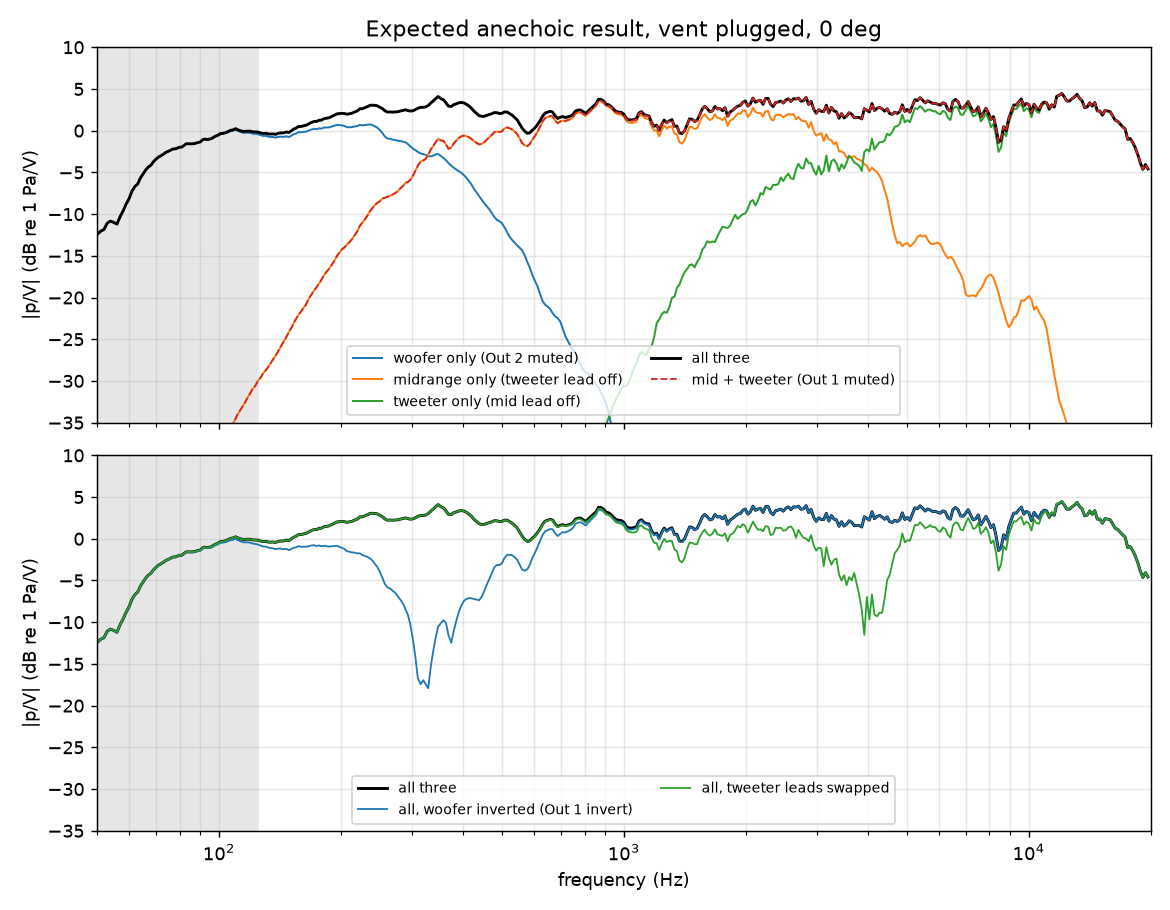
\includegraphics[width=0.8\textwidth]{expected_on.png}
\caption{Expected result at \ang{0}. Top: R1 and R2 states (woofer only, mid+tweeter, midrange only,
tweeter only, all). Bottom: R3 states (all, woofer inverted, tweeter swapped) with the notches at
\SI{329}{Hz} ($-21$~dB) and \SI{3.9}{kHz} ($-14$~dB).}\label{fig:on}
\end{figure}

\begin{figure}[H]
\centering
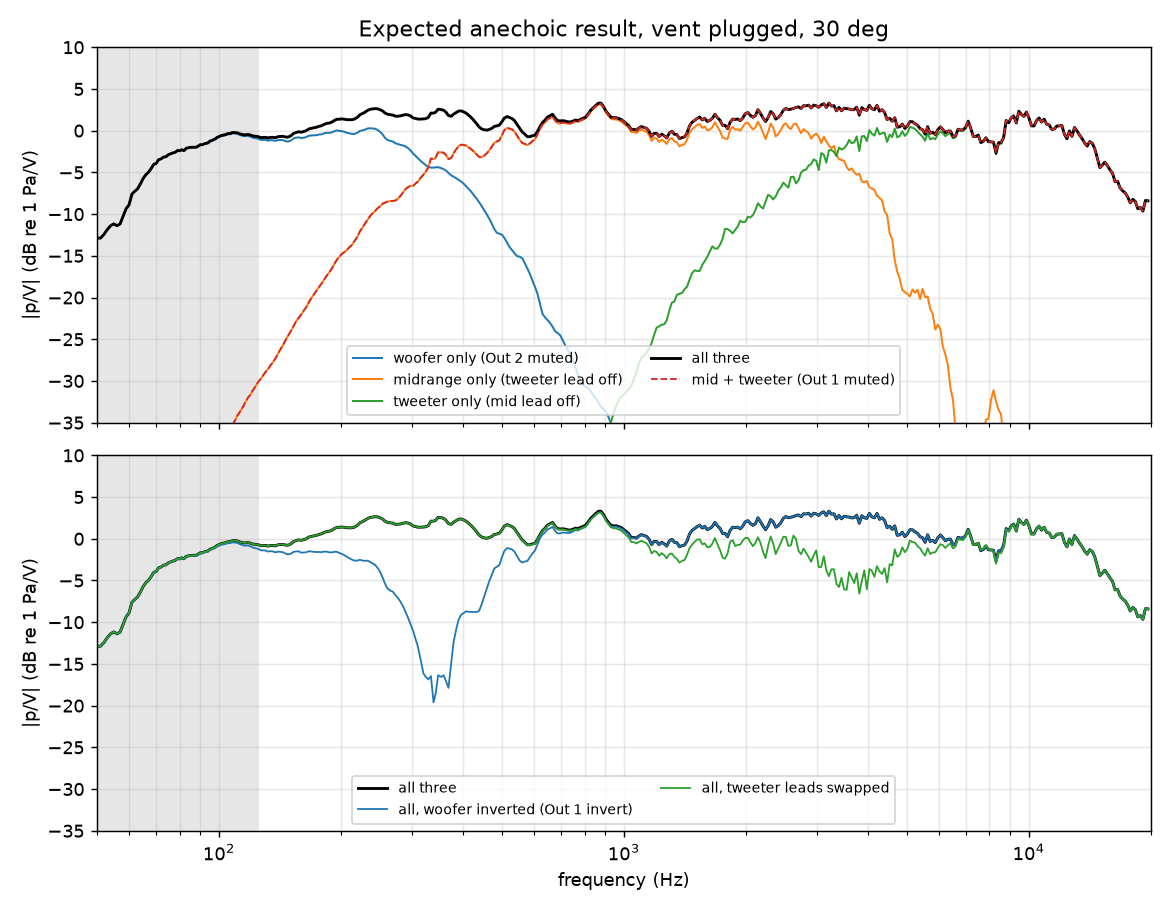
\includegraphics[width=0.8\textwidth]{expected_off30.png}
\caption{Expected result at \ang{30} (R4). Sum spread \SI{6.3}{dB} from \SI{150}{Hz} to \SI{15}{kHz}.}
\label{fig:off}
\end{figure}

\begin{figure}[H]
\centering
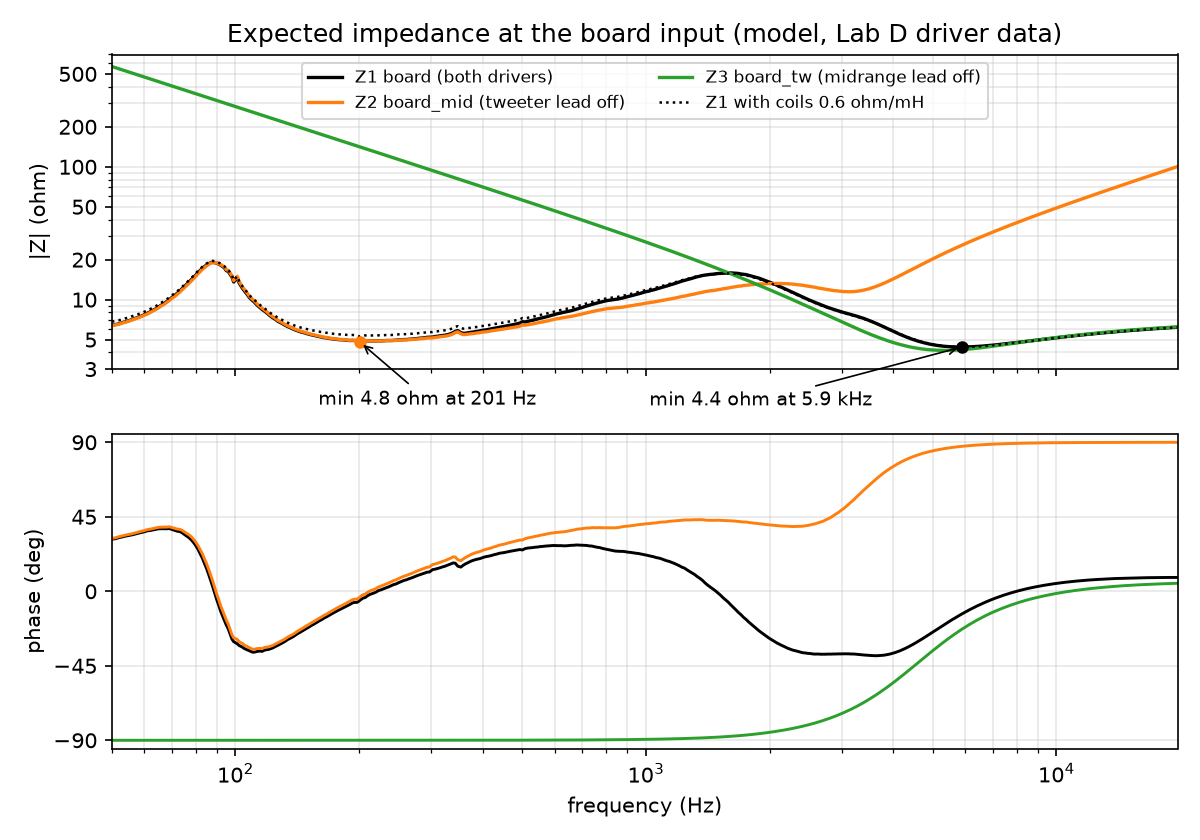
\includegraphics[width=0.72\textwidth]{expected_zi_log.png}
\caption{Expected impedance at the board input for Z1--Z3 (log scale; same data as
\file{model/expected_zi.png}). Dotted: coils with \SI{0.6}{\ohm/mH} resistance, which raises the low end
by about \SI{0.4}{\ohm}.}\label{fig:zi}
\end{figure}

% ======================================================================
\appendix
\needspace{12\baselineskip}
\section{Troubleshooting}
{\small
\begin{longtable}{@{}p{0.40\textwidth}p{0.555\textwidth}@{}}
\toprule
Symptom & What to do \\
\midrule\endhead
``No Umik'' / microphone not found & Close MATLAB, check the UMIK USB cable, start MATLAB again (the device is only
  registered at start-up). \\
``beeps.wav not found'' & \cmd{cd} into \file{Labs/Lab E/matlab/course} and run from there, or copy
  \file{Beeps.wav} next to \file{project_run.m}. \\
\cmd{test_project} / \cmd{test_zinf} not PASS & The copy of \file{Labs/} is incomplete: copy the whole folder again. \\
``Unknown state(s)'' & A typo in a state name. Valid: \cmd{woofer midtw mid tw all flipW flipT}. \\
Warning: time signal near full scale & Turn the amplifier down. Before R1: fine. During the series: redo from R1,
  since the volume must be the same for all runs. \\
Warning: UMIK signal very small & A mute left on, a lead off, the amplifier too low, or the UMIK cable. \\
Woofer -- midtw offset more than \SI{\pm1}{dB} & Change the Output 1 gain by the printed amount, note it
  (\cmd{d.minidsp_out1_gain}), repeat R1. \\
Sum check above \SI{0.5}{dB} & Something changed between states (a lead, a mute, someone in the chamber):
  repeat the run. \\
No notch, or in the wrong place, in R3 & Polarity: red to $+$ on both drivers? Invert really ticked/unticked?
  Tweeter swapped in the third state only? \\
mid+tw far from the model, woofer fine & Board wiring: run R2 to find which branch. \\
Scope: Out 1 about \SI{-29}{dB}, Out 2 about \SI{-0.5}{dB} at \SI{325}{Hz} & The MiniDSP runs at
  \SI{48}{kHz}: the coefficients put the crossover at \SI{162}{Hz}. Ask Vicente. \\
Scope: Out 1 and Out 2 equal & The \SI{-4.5}{dB} gain on Output 1 is not set. \\
Scope: outputs in opposite phase & An Invert box is ticked, or a filter text went into the wrong output. \\
``Give the measured series resistor'' & Set \cmd{R} in \file{zinf_run.m} section 0 to the multimeter value
  (20--50~$\Omega$). \\
Warning: samples on the \SI{\pm10}{V} rail & Turn the amplifier down; that run is not usable, repeat it. \\
Message ``AI0 is on a DC offset \ldots\ k = 2'' & Expected (as in Lab D). Check $|Z|$ at low frequency
  against the multimeter. \\
Board level off by more than \SI{1.5}{dB} & Wrong $R$, wrong $k$, or a lead on the wrong terminal. \\
Board $|Z|$ min below \SI{3.5}{\ohm} & A short, or both branches on the same driver. \\
Woofer $f_b$ far from \SI{23.4}{Hz} & Vent length, the second vent not plugged, filling moved. \\
Near-field level far from Lab D & Nexus not at \SI{1}{V/Pa}, microphone plugged in after the Nexus was on,
  resistor not shorted, or a very different mic distance. \\
\bottomrule
\end{longtable}
}

\section{The hand-written logbook: \file{project_dims.m}}\label{app:dims}
Every data file stores a copy of this function's output, so fill it in before the first run and update it
when something changes. NaN or empty means ``not noted yet''. Lengths in metres.

{\small
\begin{longtable}{@{}p{0.27\textwidth}p{0.68\textwidth}@{}}
\toprule
Field & What to write \\
\midrule\endhead
\cmd{UmikSN} & UMIK serial from the label (0329, 0332 or 0335); Lab E was \cmd{'708-0332'} \\
\cmd{T_celsius} & chamber temperature \\
\cmd{r_mic}, \cmd{h_mic} & front of the boxes to the microphone; microphone height (Lab E: 2.44, 1.15) \\
\cmd{layout} & where the mid/tweeter box sits on the woofer box \\
\cmd{vents}, \cmd{filling}, \cmd{dust_cover} & preset: both plugged, filling in; dust cover as in Lab E \\
\cmd{ref_channel} & confirm with Vicente: line-out looped to line-in, before the MiniDSP \\
\cmd{amp_volume}, \cmd{amp_balance} & knob position(s); how the two channels were checked equal \\
\cmd{panel_no} & passive filter panel number (1--10) \\
\cmd{minidsp_cfg} & configuration slot / saved file name \\
\cmd{minidsp_in_gain} & input gain in dB \\
\cmd{minidsp_out1_gain}, \cmd{..._out2_gain} & $-4.5$ and 0 dB (update if R1 changes it) \\
\cmd{minidsp_invert}, \cmd{minidsp_fs} & ``none''; sample rate shown in the plugin (96 kHz) \\
\cmd{board} & measured value of each of the six parts (LCR meter), next to the nominal \\
\cmd{coil_dcr} & DC resistance of $L_\mathrm{mid}$ and $L_\mathrm{tw}$ (multimeter) \\
\cmd{R_series} & series resistor at the Zi/Nfield station, multimeter (Lab D: 32.9) \\
\cmd{Rdc_board} & multimeter across the board input, drivers connected (about \SI{5}{\ohm}) \\
\cmd{vent1}, \cmd{vent2} & inner diameter and length of vent 1; vent 2's diameter and telescope range \\
\cmd{vent_used}, \cmd{nf_mic_dist} & vent setting at the Zi/Nfield station; mic distance in the near field \\
\cmd{notes} & anything else (who did what, odd events, changes) \\
\bottomrule
\end{longtable}
}

\needspace{20\baselineskip}
\section{MiniDSP filter texts}\label{app:dsp}
For reference only: \textbf{paste from the \file{.txt} files} in \file{Labs/Project/Final design/data/dsp/},
not from this PDF. The MiniDSP's $a_1$, $a_2$ have the opposite sign of the textbook form, as
\file{DigitalCrossover.m} prints them ($a_1 = +1.9699$). Both biquads are identical in each file:
two cascaded Butterworth sections ($Q = 0.707$) at \SI{325}{Hz}, $f_s = \SI{96}{kHz}$, make one LR4 filter.

\begin{minipage}[t]{0.48\textwidth}
\raggedright\textbf{Output 1, woofer:}\\ \file{MiniDSP_woofer_out1.txt}
\VerbatimInput[fontsize=\footnotesize,frame=single,framesep=1.5mm]{../../data/dsp/MiniDSP_woofer_out1.txt}
\end{minipage}\hfill
\begin{minipage}[t]{0.48\textwidth}
\raggedright\textbf{Output 2, mid + tweeter:}\\ \file{MiniDSP_midtw_out2.txt}
\VerbatimInput[fontsize=\footnotesize,frame=single,framesep=1.5mm]{../../data/dsp/MiniDSP_midtw_out2.txt}
\end{minipage}

\end{document}
